% ============================================================================
% slides.tex --- 30-minute thesis presentation
% Rewiring the market time clock in Spanish electricity markets
% Pablo Paramio Perez, CEMFI Master in Economics and Finance, June 2026
% Slides are cues, not text-walls. Verbal explanation carries the detail.
% ============================================================================

\documentclass[10pt,aspectratio=169]{beamer}

\usetheme{default}
\usecolortheme{seahorse}
\useinnertheme{circles}
\useoutertheme{infolines}
\setbeamertemplate{navigation symbols}{}
\setbeamerfont{frametitle}{size=\large,series=\bfseries}
\setbeamercolor{frametitle}{fg=black,bg=blue!10}
\setbeamerfont{title}{size=\Large,series=\bfseries}
\setbeamercolor{title}{fg=blue!50!black}
\setbeamercolor{structure}{fg=blue!50!black}

\usepackage{amsmath,amssymb}
\usepackage{graphicx}
\usepackage{booktabs}
\usepackage{multirow}
\usepackage{tikz}
\usepackage{dsfont}
\usetikzlibrary{arrows.meta,positioning,decorations.pathreplacing}
\usepackage{xcolor}
\usepackage{colortbl}
\usepackage[round,authoryear]{natbib}
\bibliographystyle{plainnat}
\graphicspath{{../../../figures/thesis/}{../../../figures/working/}}

% Section divider slides
\AtBeginSection[]{
  \begin{frame}[plain]
    \vfill
    \begin{center}
      {\large\color{gray!60!black}Part \insertsectionnumber}\\[0.6cm]
      {\Huge\bfseries\color{blue!50!black}\insertsection}
    \end{center}
    \vfill
  \end{frame}
}

\title[Granularity in Spanish electricity markets]{Rewiring the market time clock in Spanish electricity markets:\\
strategic behaviour and market power with higher granularity}
\author[Pablo Paramio P\'erez]{Pablo Paramio P\'erez}
\institute[CEMFI]{CEMFI Master in Economics and Finance}
\date{June 2026}

\begin{document}

% ---------------------------------------------------------------------------
\begin{frame}[plain]
\titlepage
\end{frame}

% ---------------------------------------------------------------------------
\begin{frame}{Outline}
\begin{enumerate}\setlength{\itemsep}{6pt}
  \item Question and headline
  \item Setting and reforms
  \item Mechanisms and identification
  \item Empirical results
  \item Conclusion
\end{enumerate}
\end{frame}

% ---------------------------------------------------------------------------
\section{Setting and reforms}

% ---------------------------------------------------------------------------
\begin{frame}{Question and headline}
\textbf{Setting.} Sequential electricity wholesale markets. Spain switched the trading time resolution from $60$ minutes to $15$ minutes in two staggered reforms in $2025$, March and October.

\bigskip
\textbf{Question.} Does finer time-resolution reshape strategic bidding? Does market power go up or down? What effect do we see in prices, market differentials, and imbalance penalties?

\bigskip
\textbf{Answer.} COMPLETE!!!

\bigskip
\textbf{Caveat.} An April $2025$ blackout triggered a separate regulatory regime that inflated the system-cost line. Granularity and that regime are calendar-overlapping but mechanistically distinct.
\end{frame}

% ---------------------------------------------------------------------------

\begin{frame}{The institutional setting --- sequential electricity wholesale markets}
\bigskip
\textbf{The product.} Delivery of MW (rate) over a fixed short time slot, by different technologies.

\bigskip
\textbf{Sequence of markets.} Electricity cannot be stored cheaply, supply must equal demand in real time. For this reason, we have sequential \textbf{wholesale} markets before delivery:
\begin{itemize}\setlength{\itemsep}{1pt}
  \item \textbf{Forward auction (``day-ahead'', DA)} --- clears the day before. Biggest market, with the most liquidity.
  \item \textbf{Spot auctions (``intraday auctions'', IDA)} --- clears closer to delivery. Corrections. 
  \item \textbf{Balancing (real time)} --- corrections by the system operator (REE). Highly complex, with separate pricing mechanisms (APPENDIX).
\end{itemize}
Both DA and IDA are \textbf{uniform-price multi-unit auctions}; bidders submit step-function supply and demand curves and price is set at the intersection of the aggregate supply and demand curves, using a complex algorithm that maximizes social welfare.

\bigskip
\textbf{Huge complexity:} ancillary markets, bilateral contracts, cross-border trading, continuous intraday markets, etc. We focus on DA and IDA, and present basic descriptive statistics on some of the rest.

\end{frame}

% ---------------------------------------------------------------------------
\begin{frame}{The Spanish reform sequence}
\centering
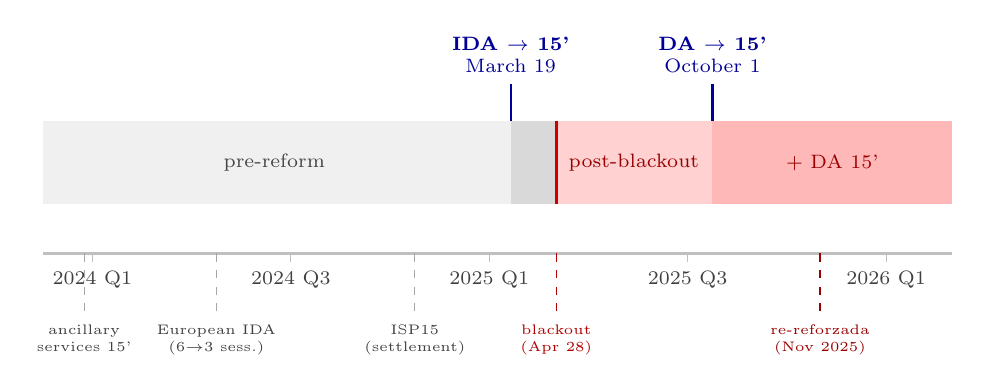
\begin{tikzpicture}[scale=1.05, every node/.style={font=\footnotesize}]
  \def\W{11.0}

  % REGIME BANDS
  \fill[gray!12]  (0.0,  0.6) rectangle (5.66, 1.6); \node[font=\scriptsize, gray!55!black] at (2.8, 1.1) {pre-reform};
  \fill[gray!30]  (5.66, 0.6) rectangle (6.21, 1.6);
  \fill[red!18]   (6.21, 0.6) rectangle (8.10, 1.6); \node[font=\scriptsize, red!60!black] at (7.15, 1.1) {post-blackout};
  \fill[red!28]   (8.10, 0.6) rectangle (\W,   1.6); \node[font=\scriptsize, red!60!black] at (9.55, 1.1) {$+$ DA 15'};

  % BLACKOUT VERTICAL LINE INSIDE BAND
  \draw[red!80!black, very thick] (6.21, 0.6) -- (6.21, 1.6);

  % BIG REFORM MARKERS (above bands)
  \draw[blue!60!black, thick] (5.66, 1.6) -- (5.66, 2.05);
  \node[anchor=south, align=center, font=\scriptsize, blue!60!black] at (5.66, 2.07) {\textbf{IDA $\to$ 15'}\\March 19};
  \draw[blue!60!black, thick] (8.10, 1.6) -- (8.10, 2.05);
  \node[anchor=south, align=center, font=\scriptsize, blue!60!black] at (8.10, 2.07) {\textbf{DA $\to$ 15'}\\October 1};

  % MAIN TIMELINE
  \draw[gray!50, thick] (0,0) -- (\W,0);
  \foreach \x/\lbl in {0.6/{2024 Q1}, 3.0/{2024 Q3}, 5.4/{2025 Q1}, 7.8/{2025 Q3}, 10.2/{2026 Q1}} {
    \draw[gray!50] (\x, 0) -- (\x, -0.10);
    \node[anchor=north, gray!50!black, font=\scriptsize] at (\x, -0.10) {\lbl};
  }

  % SMALL TICKS BELOW (pre-reforms, blackout, re-reforzada)
  \foreach \x/\lbl in {0.5/{ancillary\\services 15'}, 2.1/{European IDA\\(6$\to$3 sess.)}, 4.5/{ISP15\\(settlement)}} {
    \draw[gray!70, dashed, thin] (\x, 0) -- (\x, -0.7);
    \node[anchor=north, align=center, font=\tiny, gray!50!black] at (\x, -0.75) {\lbl};
  }
  \draw[red!70!black, dashed, thin] (6.21, 0) -- (6.21, -0.7);
  \node[anchor=north, align=center, font=\tiny, red!70!black] at (6.21, -0.75) {blackout\\(Apr 28)};
  \draw[red!60!black, dashed, thin] (9.4, 0) -- (9.4, -0.7);
  \node[anchor=north, align=center, font=\tiny, red!60!black] at (9.4, -0.75) {re-reforzada\\(Nov 2025)};
\end{tikzpicture}

\vspace{0.4cm}
\begin{itemize}
  \item \textbf{Main reforms.} Change in time granularity of \textbf{IDA} (March 2025) and \textbf{DA} (October 2025): from $60$-min products to $15$-min.
  \item \textbf{Other pre-reforms in 2024}: ancillary services, European IDAs, imbalance quarter-hourly settlement.
  \item \textbf{April 2025 blackout} that triggered separate regulatory regime ("operaci\'on reforzada", later "re-reforzada").
\end{itemize}

\end{frame}

% ---------------------------------------------------------------------------

\begin{frame}{Literature review}
\footnotesize

\textbf{Sequential markets, forward contracts, Cournot.}
\citet{allaz_vila_1993}; \citet{ito_reguant_2016}.

\medskip
\textbf{Empirical bidding in multi-unit electricity auctions.}
\citet{hortacsu_puller_2008}; \citet{hortacsu_luco_puller_zhu_2019}.

\medskip
\textbf{Trading-granularity and settlement-period reforms.}
\citet{markle_huss_2017}; \citet{csereklyei_khezr_2024}.

\medskip
\textbf{Renewable price impacts and ancillary services in Spain.}
\citet{brown_reguant_2026}.

\medskip
\textbf{Iberian blackout and post-blackout regime.}
\citet{davi_arderius_graf_2026}; \citet{entsoe_blackout_iberia_2026}; \citet{cnmc_blackout_recommendations_2026}.

\end{frame}

% ---------------------------------------------------------------------------
\section{Mechanisms and identification strategy}

\begin{frame}{A priori mechanisms expected from the reform sequence}
\begin{itemize}
  \item We expect production to shift to the granular side of the market.... MORE FOR RENEWABLES. This effect would be bigger for ID15 into the IDAs, since it is near delivery, and greater the bigger the shocks volatility between DA and IDA are.
  \item If residual demand of the price setter firms gets more inelastic in each quarter (thinner market), we expect prices to increase. If it gets more elastic, the opposite
  \item CHANGE IN THE BID SHAPE WITH THE REFORM: MORE VARIATION IN TRANCHES, MORE DETAIL, LESS AGGREGATION.
\end{itemize}
\end{frame}

% ---------------------------------------------------------------------------
\begin{frame}{Data architecture}
I build from scratch a \textbf{full automated data pipeline} for the public market data, using 3 sources:
\medskip
\begin{itemize}
  \item \textcolor{olive}{Wholesale market operator data (OMIE):} DA and IDA prices, auction quantities, bilaterals, accepted bid-curves, etc. Continuos market is included too, but not the focus.
  \item \textcolor{cyan}{System operator data (REE) via their API:} balancing market prices, ancillary services, etc.
  \item \textcolor{violet}{European data portal (ENTSO-E) via API:} cross-border flows, wind and solar production, etc. 
\end{itemize}
\bigskip
\textbf{Magnitude.} 420GB of raw data, 200GB processed in \textit{parquet} format. Around 10 billion rows. Dedicated external SSD for storage and processing.

\bigskip
\textbf{Time window.} January 2018 -- today, idempotent code. Different granularities across time.

\end{frame}



% ---------------------------------------------------------------------------
\begin{frame}{Bid-curve variables}
\begin{columns}[T]
\begin{column}{0.50\textwidth}
\centering
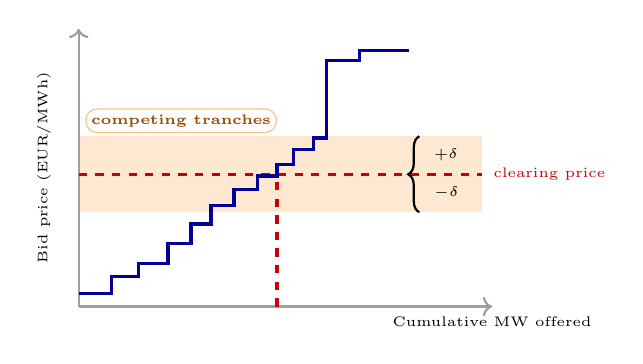
\begin{tikzpicture}[scale=0.42, every node/.style={font=\tiny}]
  \def\xmax{12.5} \def\ymax{8.4} \def\mcp{4} \def\h{1.15} \def\ceiling{6.6}
  \fill[orange!18] (0, \mcp-\h) rectangle (\xmax-0.3, \mcp+\h);
  \draw[->, thick, gray!75] (0,0) -- (\xmax,0) node[below, black]{Cumulative MW offered};
  \draw[->, thick, gray!75] (0,0) -- (0,\ymax);
  \node[rotate=90, anchor=south, black] at (-0.55, \ymax/2){Bid price (EUR/MWh)};
  \draw[red!80!black, very thick, dashed] (0, \mcp) -- (\xmax-0.3, \mcp);
  \node[red!80!black, anchor=west] at (\xmax-0.25, \mcp){clearing price};
  \draw[blue!60!black, very thick]
       (0, 0.4) -- (1, 0.4) -- (1, 0.9) -- (1.8, 0.9) -- (1.8, 1.3) -- (2.7, 1.3)
    -- (2.7, 1.9) -- (3.4, 1.9) -- (3.4, 2.5) -- (4, 2.5) -- (4, 3.05) -- (4.7, 3.05)
    -- (4.7, 3.55) -- (5.4, 3.55) -- (5.4, 3.95) -- (6, 3.95) -- (6, 4.30) -- (6.5, 4.30)
    -- (6.5, 4.75) -- (7.1, 4.75) -- (7.1, 5.10) -- (7.5, 5.10) -- (7.5, 7.45) -- (8.5, 7.45)
    -- (8.5, 7.75) -- (10, 7.75);
  \draw[red!80!black, very thick, dashed] (6, 0) -- (6, \mcp);
  \draw[decorate, decoration={brace, amplitude=4pt, mirror}, thick]
    (\xmax-2.2, \mcp+\h) -- (\xmax-2.2, \mcp-\h);
  \node[anchor=west] at (\xmax-2.05, \mcp+\h/2){$+\delta$};
  \node[anchor=west] at (\xmax-2.05, \mcp-\h/2){$-\delta$};
  \node[orange!60!black, anchor=south west, fill=white, rounded corners, inner sep=2pt, draw=orange!50]
    at (0.2, \mcp+\h+0.10) {\textbf{competing tranches}};
\end{tikzpicture}

\medskip
\footnotesize
Not all tranches of the bid curves are equally relevant for strategic bidding, we focus on \textbf{tranches around clearing price in that period}, using a bandwidth:
\begin{equation*}
\mathcal{B}_{u,d,p} = \{k: |p_k - \text{MCP}_{d,p}| \leq \delta \}.
\end{equation*}
choosing the bandwidth $\delta = p_{90} - p_{50}$ in the time-window of interest. Note that both the level and the width of $\mathcal{B}_{u,d,p}$ vary across time!
\end{column}

\begin{column}{0.50\textwidth}

\textbf{Bid-curve shape measures:}
\begin{itemize}\setlength{\itemsep}{10pt}\setlength{\parskip}{3pt}
  \item Slope and level of the bid curve: for each curve, fit $p_k = \hat{\alpha} + \hat{\beta} Q_k$ in $k\in\mathcal{B}$ and get $(\hat{\alpha}, \hat{\beta})$.
  Similar with the 2nd order polynomial to get the curvature $\tilde{\gamma}$.
  \item Robust measures to few tranches inside the band:
  \begin{itemize}\setlength{\itemsep}{8pt}\setlength{\parskip}{3pt}
    \item Quantity-weighted Herfindahl over tranches: $\text{HHI}_p = \sum_{k\in\mathcal{B}} w_k^2$, with weights $w_k = \frac{q_k}{\sum_{j\in\mathcal{B}} q_j}$.
    \item Quantity-weighted SD of tranche prices: $\sigma_p = \sqrt{\sum_{k\in\mathcal{B}} w_k (p_k - \bar p)^2}$, where $\bar p = \sum_{k\in\mathcal{B}} w_k p_k$.
  \end{itemize}

\end{itemize}

\end{column}
\end{columns}
\end{frame}

% ---------------------------------------------------------------------------

\begin{frame}{Residual demand and hour classification}

\begin{center}
\fcolorbox{blue!50!black}{blue!7}{%
\begin{minipage}{0.96\linewidth}\vspace{2pt}
\textbf{\color{blue!50!black}Key idea.} Granularity is useful when there is variation in the residual demand for each firm, and particularly for the strategic bidders. Renewable producers exploit granularity due to operational reasons (forecast updates).
\vspace{2pt}\end{minipage}}
\end{center}

\bigskip
We calculate the residual demand as the thermal gap: final program net of realized wind and solar generation, $\text{RD}(q,h,d) = [\text{load}-\text{wind}-\text{solar}]_{q,h,d}$, observed at quarter-hour resolution since 2024. To make the comparison scale-free we use the \textbf{coefficient of variation} $\mathrm{CV}(h)=\mathbb{E}_d[\text{sd}_q(\text{RD}(q,h,d))]/\mathbb{E}_d[\overline{\text{RD}}(h,d)]$, and split the hours of the day into three classes:

\medskip
\begin{itemize}\setlength{\itemsep}{4pt}
\item $\left.\begin{array}{@{}l@{}}
\textbf{Morning ramp } \mathcal{C}_M\text{: } \mathrm{CV}\approx 6.0\%\ (4.0\times\text{ flat}) \\[2pt]
\textbf{Evening ramp } \mathcal{C}_E\text{: } \mathrm{CV}\approx 3.8\%\ (2.5\times\text{ flat})
\end{array}\right\}\ \textbf{Critical }\mathcal{C}=\mathcal{C}_M\cup\mathcal{C}_E,\ \overline{\mathrm{CV}}\approx 4.6\%\ (3.1\times\text{ flat})$
\item \textbf{Flat} $\mathcal{F}$, deep night hours, $\mathrm{CV}\approx 1.5\%$ (baseline).
\item \textbf{Midday} $\mathcal{M}$, $\mathrm{CV}\approx 5.7\%$ ($3.8\times$ flat).
\end{itemize}

\end{frame}

% ---------------------------------------------------------------------------

\begin{frame}{Identification strategy: bid-curve shape}

\begin{center}
\fcolorbox{blue!50!black}{blue!7}{%
\begin{minipage}{0.96\linewidth}\vspace{4pt}
\textbf{Identification for bid-curve shape.} Check evolution of bid-curve shape measures in critical hours vs flat hours, pre vs post reform, to measure the effect of granularity on bid shape.

\medskip
\textbf{Why use a DiD here?} It differences out across-hour changes in bidding complexity, such as more advanced software, prediction models, etc.
\vspace{4pt}\end{minipage}}
\end{center}

\bigskip
\textbf{\textcolor{red}{Caveat: flat hours are not a perfect controls.}} They are also affected by the reform, but economic theory tells us that the biggest effects of the reform are in critical hours $\to$ \textbf{lower bound of the effect.}

\bigskip
The identification assumption is the usual \textbf{parallel trends:} absence granularity reform, the evolution of the bid shape of critical and flat hours would have been the same. 

\bigskip
Note that our bid-curve shape measures are robust to seasonal level changes! Main threat: post-reform shocks that affect differently critical vs flat hours, not present before.

\end{frame}

% ---------------------------------------------------------------------------

\begin{frame}{Identification strategy: level variables}
  For level variables like prices, quantities, etc, \textbf{seasonality} is the big issue, since changes in renewable production affect differently critical and flat hours across the year.

  \bigskip
  Moreover, for quantity variable we have to be very very catious and interpret correctly the different programs and REE restrictions.

  \bigskip
  Following previous work of the EPEX reform \citep{markle_huss_2017} we use Bayesian Structural Time Series \citep{brodersen_2015} and standard OLS exploiting all the rich data and granularity.

  \bigskip
  The most important part is the choice of windows and controls:
  \begin{itemize}
     \item \textbf{Windows.} We use a long pre-window from 2022 to capture full seasonality across years. The other alternative is to use reforzada-constant windows, or excluding periods with different regimes but that would reduce the pre-window length and thus the ability to capture seasonality and real renewable growth.
    \item \textbf{Controls.} We control for wind and solar production, and gas price, which are the main drivers of price variation in the Spanish market. We also include year-by-year interactions to capture the growth in renewables, which crucial to get depressing effect in prices of solar in midday hours.
  \end{itemize}

\end{frame}


% ---------------------------------------------------------------------------
\section{Empirical results}

\begin{frame}{Summary of our results}
  For ID15:
  \begin{itemize}
    \item Decrease in prices in both IDA and DA after controlling for renewable penetration and seasonality. Price wedge between DA and IDAs increase.
    \item No change in aggregate volume, wind sells more actively in IDA. Nuclear was out of the market post-ID15 and pre-blackout. SELL SHARE HERE.
    \item BID SHAPE HERE. RESIDUAL DEMAND HERE.
  \end{itemize}

  For DA15:
  \begin{itemize}
    \item Small decrease in DA prices, null in IDA, after controlling for renewable penetration and seasonality. Price wedge do not vary.
    \item AGGREGATE QUANTITIES HERE. TECH VARIATION HERE. SELL SHARE HERE.
    \item BID SHAPE HERE. RESIDUAL DEMAND HERE.
  \end{itemize}
\end{frame}


% ---------------------------------------------------------------------------
\subsection{Prices, wedge, and quantity}

\begin{frame}{Prices --- robust drop at ID15, null at DA15}
\footnotesize
\centering
\setlength{\tabcolsep}{6pt}
\begin{tabular}{l c c c c}
\toprule
                                                   & \multicolumn{2}{c}{\textbf{ID15 (IDA reform)}} & \multicolumn{2}{c}{\textbf{DA15 (DA reform)}} \\
\cmidrule(lr){2-3}\cmidrule(lr){4-5}
                                                   & IDA (own) & DA (cross) & DA (own) & IDA (cross) \\
\midrule
OLS daily --- base (month $+$ DOW)                   & \cellcolor{green!22}$-32^{***}$ & \cellcolor{green!22}$-33^{***}$ & \cellcolor{red!18}$-8$ & \cellcolor{red!18}$-8$ \\
OLS daily --- $+$ year-by-renewable (per year)       & \cellcolor{green!22}$-46^{***}$ & \cellcolor{green!22}$-47^{***}$ & \cellcolor{red!18}$\mathbf{-9}$ & \cellcolor{red!18}$\mathbf{-10}$ \\
OLS daily --- $+$ year-by-renewable (2024+25 pooled) & \cellcolor{green!22}$\mathbf{-39}^{***}$ & \cellcolor{green!22}$\mathbf{-39}^{***}$ & \cellcolor{red!18}$-5$ & \cellcolor{red!18}$-6$ \\
\addlinespace
OLS hourly --- base (hour $+$ month $+$ DOW)         & \cellcolor{green!22}$-34^{***}$ & \cellcolor{green!22}$-34^{***}$ & \cellcolor{red!18}$-10^{*}$ & \cellcolor{red!18}$-10^{*}$ \\
OLS hourly --- $+$ year-by-renewable (per year)      & \cellcolor{green!22}$-40^{***}$ & \cellcolor{green!22}$-39^{***}$ & \cellcolor{red!18}$-3$ & \cellcolor{red!18}$-4$ \\
OLS hourly --- $+$ year-by-renewable (2024+25 pooled)& \cellcolor{green!22}$\mathbf{-30}^{***}$ & \cellcolor{green!22}$\mathbf{-29}^{***}$ & \cellcolor{red!18}$3$ & \cellcolor{red!18}$2$ \\
\addlinespace
BSTS daily                                           & \cellcolor{green!22}$-34^{*}$ & \cellcolor{green!22}$-34^{*}$ & \cellcolor{red!18}$8$ & \cellcolor{red!18}$1$ \\
\bottomrule
\end{tabular}

\smallskip
{\scriptsize\itshape Window 2022-01-01 onward: preblackout for ID15 (40 days), 90 days for DA15. \textbf{Base controls} (all rows): wind, solar, gas, calendar-month FE, day-of-week FE. Newey-West HAC SE. We average quarter-hour prices.}

\medskip
\raggedright
\begin{itemize}\setlength{\itemsep}{1pt}
  \item \textcolor{green!40!black}{\textbf{ID15 own-venue price drop is robust} at $-30$ to $-46$ EUR/MWh across all specs}; cross-market response on DA is the same magnitude (anticipation through backward induction).
  \item \textcolor{red!70!black}{\textbf{DA15 own-venue null}} ($-9$ to $+8$); cross-market also null.
  \item \textbf{ID15 effect persists at the 90-day post-window, including blackout} (OLS pooled $-42^{***}$, BSTS real effect $-35$ EUR/MWh) --- full sensitivity at 40d / 90d / 180d / 196d in appendix.
  \item \textbf{Effect is broadly uniform across hour classes at ID15}: evidence of hydro-pump and batteries arbitrage (CHECK BID SHAPE!!!).
\end{itemize}
\end{frame}


\begin{frame}{Price wedges --- per-IDA-session levels and wedge SD}
\scriptsize
\centering
\textbf{(a) Wedge level per session} (EUR/MWh; $p_{\text{DA}} - p_{\text{IDA},s}$; pre 2024-06-14$+$, Newey-West HAC).
\smallskip
\setlength{\tabcolsep}{3pt}
\begin{tabular}{l c c c c c c}
\toprule
                                                   & \multicolumn{3}{c}{\textbf{ID15 (IDA reform)}} & \multicolumn{3}{c}{\textbf{DA15 (DA reform)}} \\
\cmidrule(lr){2-4}\cmidrule(lr){5-7}
                                                   & S1 & S2 & S3 & S1 & S2 & S3 \\
\midrule
OLS daily --- base (month $+$ DOW)                   & \cellcolor{green!22}$2.8^{**}$  & $-0.1$ & \cellcolor{red!18}$-9.6^{**}$ & $0.3$  & $-2.8$ & $2.8$ \\
OLS daily --- $+$ year-by-renewable (per year)       & \cellcolor{green!22}$2.9^{**}$  & $-0.4$ & \cellcolor{red!18}$-7.7^{*}$  & $-0.1$ & $-3.6$ & $2.3$ \\
OLS daily --- $+$ year-by-renewable (2024+25 pooled) & \cellcolor{green!22}$3.0^{**}$  & $0.3$  & \cellcolor{red!18}$-7.0^{*}$  & $0.0$  & $-2.4$ & $3.7$ \\
\addlinespace
OLS hourly --- base (hour $+$ month $+$ DOW)         & \cellcolor{green!22}$2.7^{**}$  & $0.7$  & \cellcolor{red!18}$-0.9$ & $1.0$  & $-3.0$ & $0.6$ \\
OLS hourly --- $+$ year-by-renewable (per year)      & \cellcolor{green!22}$2.8^{**}$  & $1.0$  & \cellcolor{red!18}$-0.7$ & $0.6$  & $-3.1$ & $1.4$ \\
OLS hourly --- $+$ year-by-renewable (2024+25 pooled)& \cellcolor{green!22}$2.8^{**}$  & $1.0$  & \cellcolor{red!18}$-0.7$ & $0.6$  & $-3.1$ & $1.4$ \\
\addlinespace
BSTS daily                                           & \cellcolor{green!22}$1.6^{**}$  & $1.5$  & \cellcolor{red!18}$-0.6$ & $0.3$  & $0.3$  & $0.0$ \\
\bottomrule
\end{tabular}

\medskip
\textbf{(b) Wedge SD effect, by hour class} (BSTS, EUR/MWh).
\smallskip
\setlength{\tabcolsep}{6pt}
\begin{tabular}{l c c c c c}
\toprule
                & Overall & Morning ramp & Midday & Evening ramp & Flat \\
                &         & (5--8)       & (11--14) & (16--22)   & (1--3) \\
\midrule
ID15            & \cellcolor{green!22}$\mathbf{1.1}^{**}$ & \cellcolor{green!22}$\mathbf{2.3}^{***}$ & \cellcolor{red!18}$-1.6^{**}$ & \cellcolor{green!22}$1.2^{*}$ & $-0.0$ \\
DA15            & $-0.1$ & $0.5$ & $-0.7$ & $-1.4$ & $-0.5$ \\
\bottomrule
\end{tabular}

\medskip
\footnotesize
\textcolor{green!40!black}{\textbf{ID15:} S1 wedge widens $+2.7$ to $+3.0$ (robust); S3 daily narrowing does \emph{not} survive hourly or BSTS. Wedge SD jump concentrates in the \textbf{morning ramp} ($+2.3^{***}$) more than the evening ramp ($+1.2^{*}$); midday \emph{compresses} ($-1.6^{**}$).} \\
\textcolor{gray!50!black}{\textbf{DA15:} no per-session restructuring and no SD effect.}
INCLUDE PLACEBOS IN APPENDIX, THEY ARE ROBUST!!
\end{frame}


\begin{frame}{Changes in quantity --- programs must be read separately}
\centering
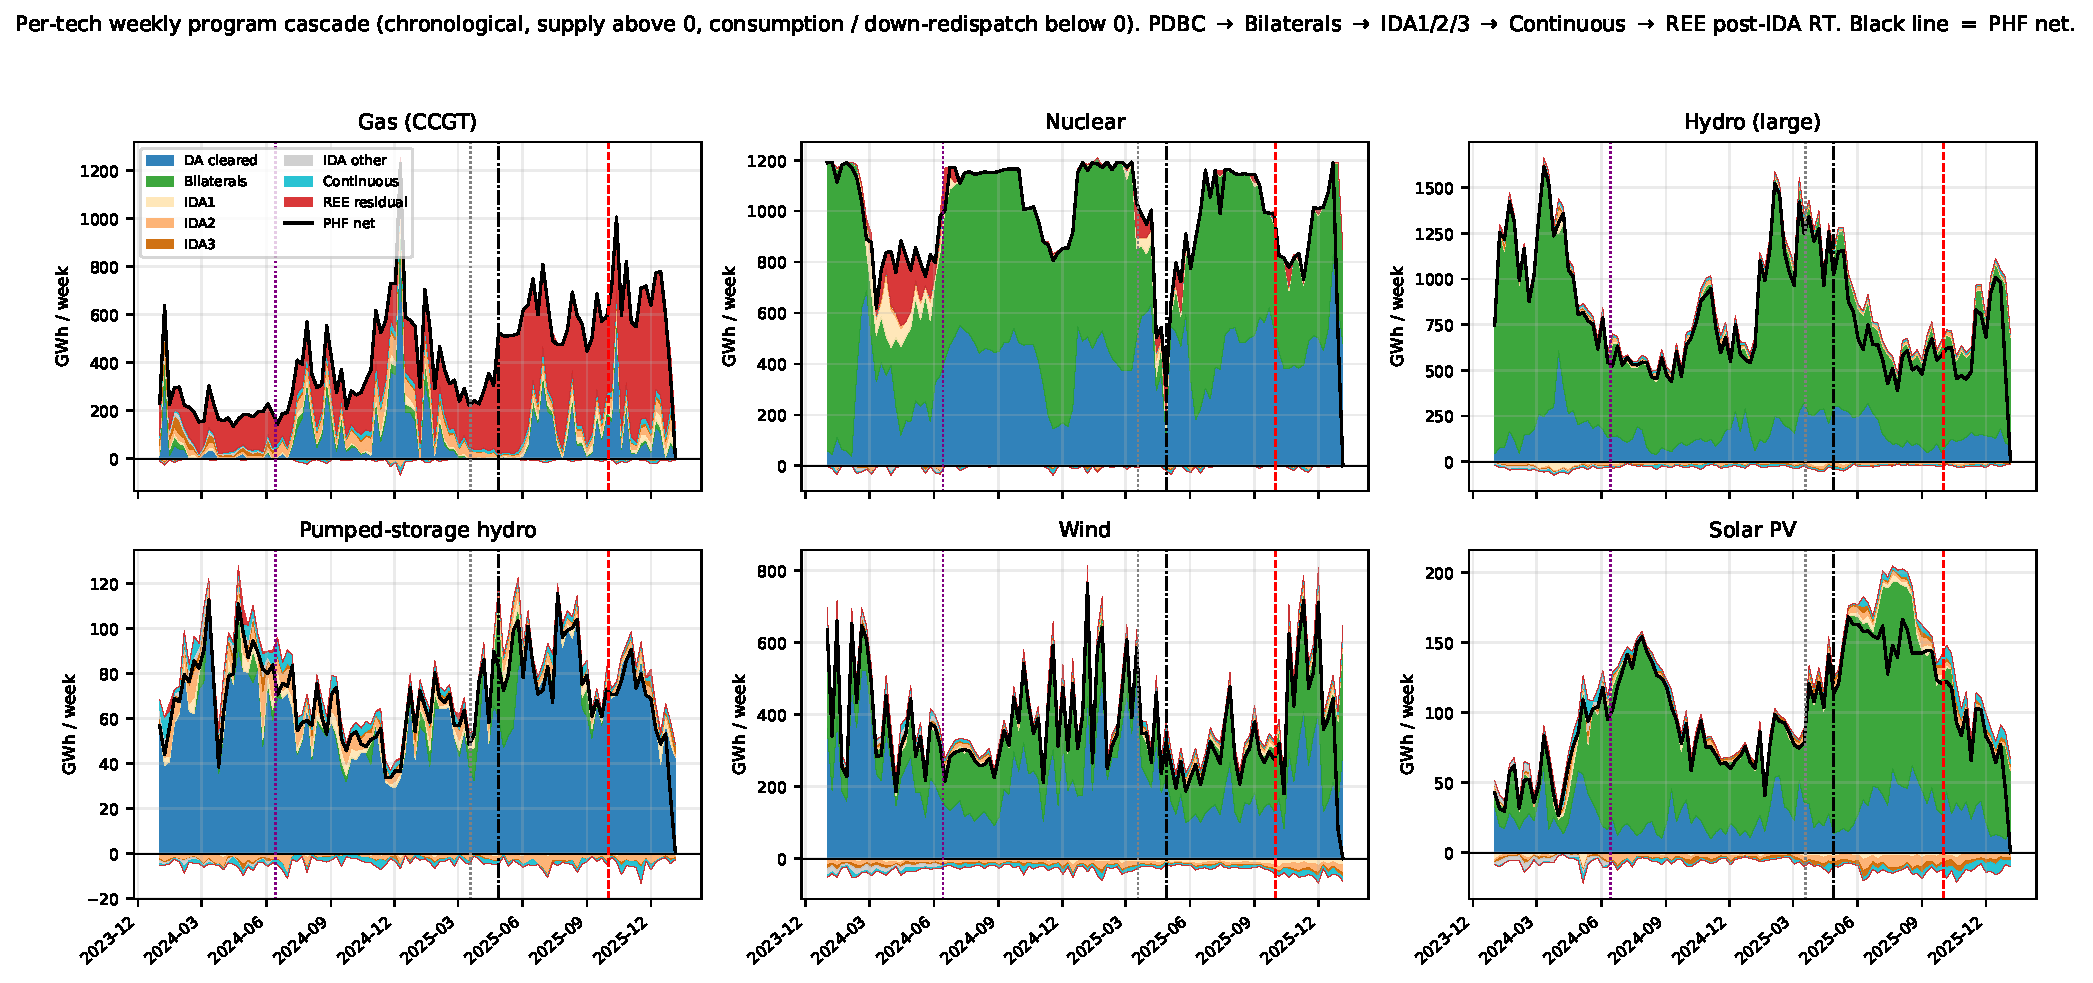
\includegraphics[width=0.96\linewidth]{fig_programs_by_tech_weekly.pdf}

\end{frame}

% ---------------------------------------------------------------------------


\begin{frame}{Changes in quantity -- main changes}
  WE SHOULD SAY QUANTITY CHANGES IN WORDS AND INCLUDE THE REGRESSIONS IN THE APPENDIX

  MENTION SELL SHARE, DROP FIGURE, NOT NEEEDED.
\end{frame}


% ---------------------------------------------------------------------------

\begin{frame}{Changes in bid shape -- critical vs flat}
  HERE FOCUS ON CCGT, HYDRO PUMP AND CHP TOO (QUITE BIG)!! PUMP STORAGE AND HYBRID ARE SMALLER BUT INTERESTING, ALSO COAL.
\end{frame}

% ---------------------------------------------------------------------------

\begin{frame}{Changes in bid shape}
  MORE HERE
\end{frame}

% ---------------------------------------------------------------------------

\begin{frame}{Changes in residual demand slope for dominant firms}
\footnotesize
\textbf{Object.} For each of the four dominant generators, the slope $b_{m,t}$ of the residual demand it faces (Cournot primitive). Steeper $\Rightarrow$ less unilateral market power.

\smallskip
\textbf{DiD spec (per firm, per reform $\times$ venue).}
\[
\log\, b_{f,t} \;=\; \theta_f\,\mathds{1}\{t \in \text{post}\} \;+\; \text{month FE} \;+\; \text{(wind, solar daily)} \;+\; \varepsilon_{f,t}.
\]
Table reports $\theta_f$ (\% change in slope).

\medskip
\centering
\setlength{\tabcolsep}{8pt}
\begin{tabular}{l c c c c}
\toprule
\textbf{Change in slope per firm} & Firm 1 & Firm 2 & Firm 3 & Firm 4 \\
\midrule
March reform, slope on IDA           & \cellcolor{green!22}$10\%$ & \cellcolor{green!22}$13\%$ & \cellcolor{green!22}$\mathbf{17}\%^{*}$ & \cellcolor{green!22}$13\%$ \\
October reform, slope on IDA         & \cellcolor{green!22}$11\%$ & \cellcolor{green!22}$13\%$ & \cellcolor{green!22}$12\%$              & \cellcolor{green!22}$\mathbf{15}\%^{***}$ \\
October reform, slope on DA          & \cellcolor{red!12}$-2\%$  & \cellcolor{red!12}$-1\%$  & \cellcolor{red!12}$-2\%$               & \cellcolor{red!12}$-3\%$ \\
\bottomrule
\end{tabular}

\medskip
\raggedright
\begin{itemize}\setlength{\itemsep}{2pt}
  \item \textcolor{green!40!black}{\textbf{Main finding (green):} slope thickens on the IDA side at both reforms.} Direction consistent for every firm; wind/solar daily-production controls barely move the coefficient $\Rightarrow$ not a supply-shift artefact.
  \item \textcolor{red!70!black}{\textbf{Negative finding (red):} DA at October.} The newly-reformed DA does NOT thicken its own slope. Effect is venue-specific to the IDA side.
\end{itemize}
\end{frame}

% ---------------------------------------------------------------------------

\begin{frame}{Elephant in the room: ancillary services}
\begin{center}
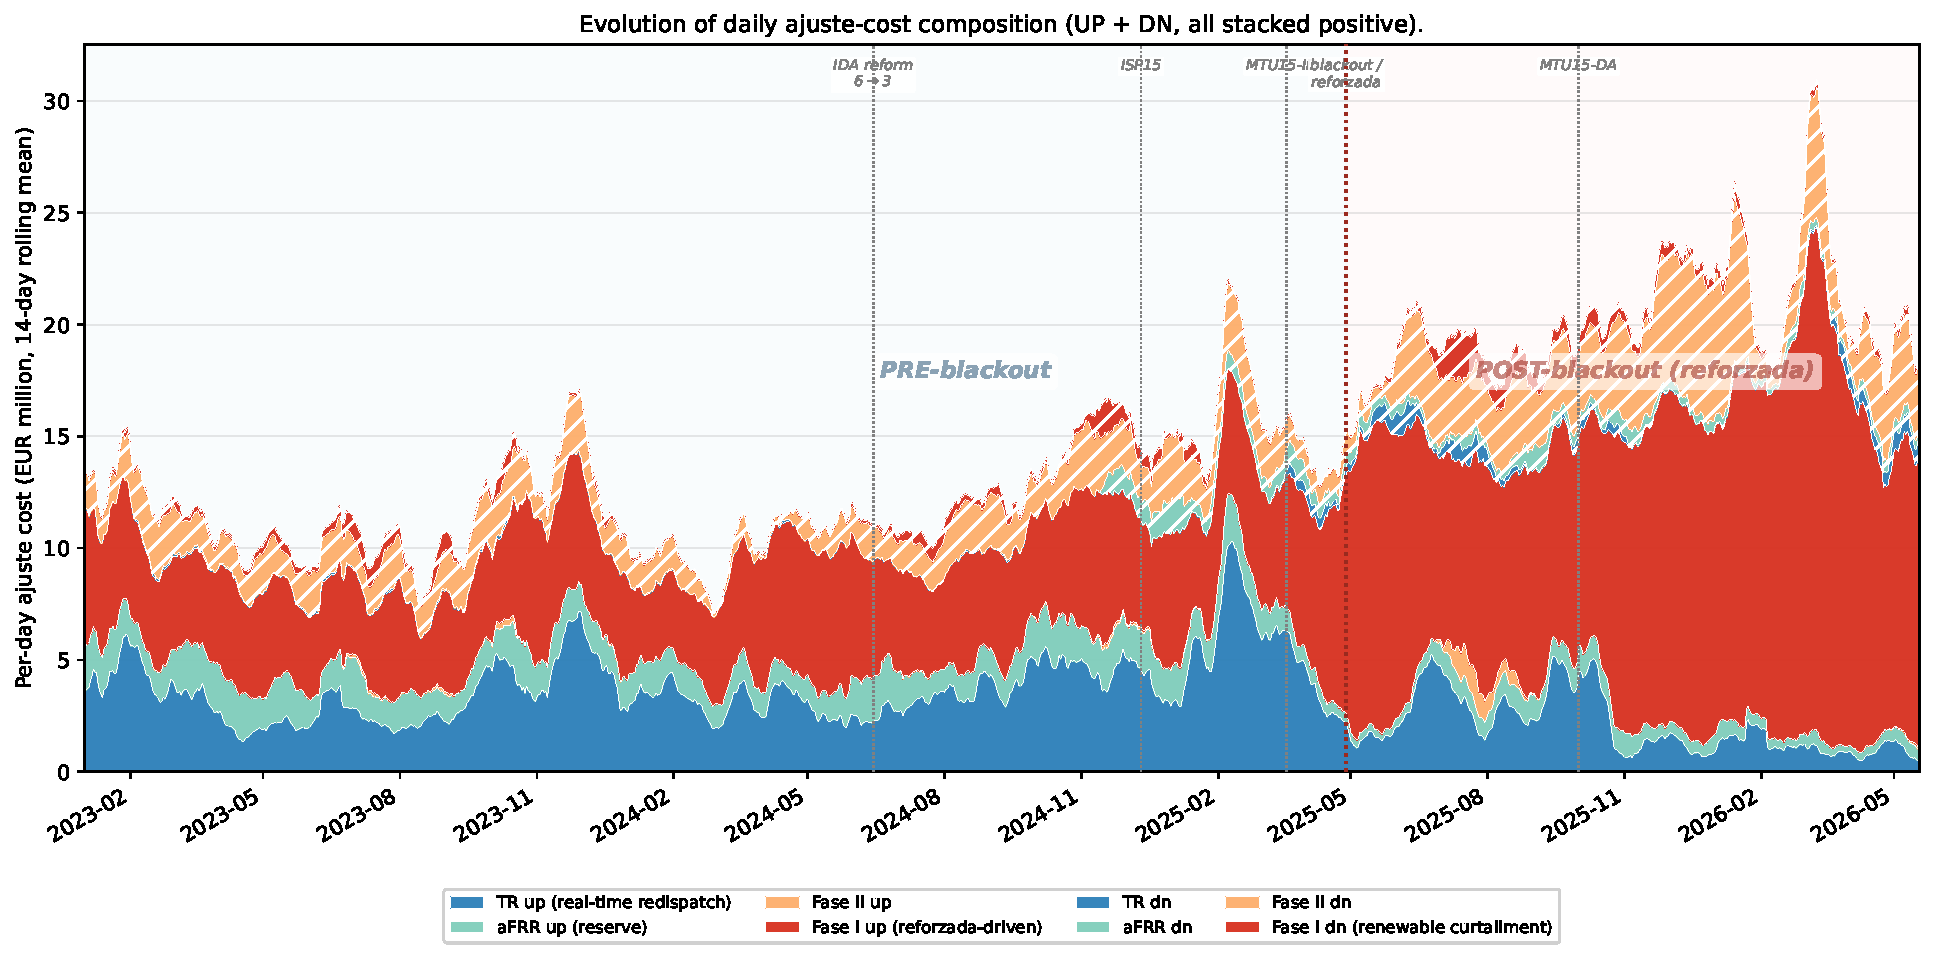
\includegraphics[width=0.72\linewidth]{efficiency_gains_timeseries.pdf}
\end{center}
\vspace{-0.1cm}
\footnotesize
\begin{itemize}\setlength{\itemsep}{2pt}
  \item The system operator is paying CCGT to produce more through adjustments in the wholesale markets, and also to solar to... stop producing. 
  \item This costs have increased substantially! QUANTITY Re-reforzada just after DA15 calls CCGT even before in the program cascade (TR up).
  \item Acknowledge by \citet{brown_reguant_2026} and \citet{davi_arderius_graf_2026}.
\end{itemize}
\end{frame}

% ---------------------------------------------------------------------------
\begin{frame}{Wedge --- mean unchanged, SD jumps, per-session restructures (ID15)}
\footnotesize
\begin{columns}[T]
\begin{column}{0.50\textwidth}
\textbf{(a) BSTS: within-day wedge SD} (Spec~A, 2024 same-calendar placebo).
\centering
\setlength{\tabcolsep}{4pt}
\begin{tabular}{l c c}
\toprule
\textbf{Wedge SD (EUR/MWh)} & \textbf{Real} & \textbf{2024 plb.} \\
\midrule
March, overall          & \cellcolor{green!22}$\mathbf{1.15}^{**}$  & \cellcolor{gray!12}$-0.96$ \\
March, peak hours       & \cellcolor{green!22}$\mathbf{2.12}^{***}$ & \cellcolor{gray!12}$-0.68$ \\
October                 & \cellcolor{green!22}$1.12$ (persists)     & \cellcolor{gray!12}$0.09$ \\
\bottomrule
\end{tabular}

\medskip
\textcolor{green!40!black}{\textbf{Wedge SD jumps at March, stays elevated through October}} --- bounded per-product arbitrage: with $4\times$ more delivery products, capacity per product binds. SD lands at $\sim 2\times$ the unconstrained benchmark, not zero.

\medskip
\textcolor{red!70!black}{\textbf{Mean unchanged}} at either reform (granularity does not collapse the level wedge).
\end{column}

\begin{column}{0.50\textwidth}
\textbf{(b) OLS: wedge level per IDA session} (Newey-West HAC, long pre 2024-06-14$+$).
\centering
\setlength{\tabcolsep}{4pt}
\begin{tabular}{l r r}
\toprule
                  & \textbf{ID15} & \textbf{DA15} \\
\textbf{Wedge}    & $\hat\theta$ (EUR/MWh) & $\hat\theta$ \\
\midrule
Aggregate         & $-0.04$  & $1.31$ \\
Session 1 (early) & \cellcolor{green!22}$\mathbf{3.0}^{**}$ & $-0.09$ \\
Session 2 (mid)   & $0.3$   & $-3.6$ \\
Session 3 (late)  & \cellcolor{red!12}$\mathbf{-7.7}^{*}$ & $2.3$ \\
\bottomrule
\end{tabular}

\medskip
\textcolor{green!40!black}{\textbf{At ID15 the wedge restructures \emph{within} day:}} S1 (early, nearer DA gate) widens $+3$; S3 (late, nearer delivery) narrows $-7.7$. Aggregate null.

\medskip
\textcolor{red!12!black}{No per-session restructuring at DA15.}
\end{column}
\end{columns}
\end{frame}


% ---------------------------------------------------------------------------
\begin{frame}{Quantity --- IDA sell-share rises at ID15 (figure + BSTS)}
\begin{columns}[T]
\begin{column}{0.55\textwidth}
\centering
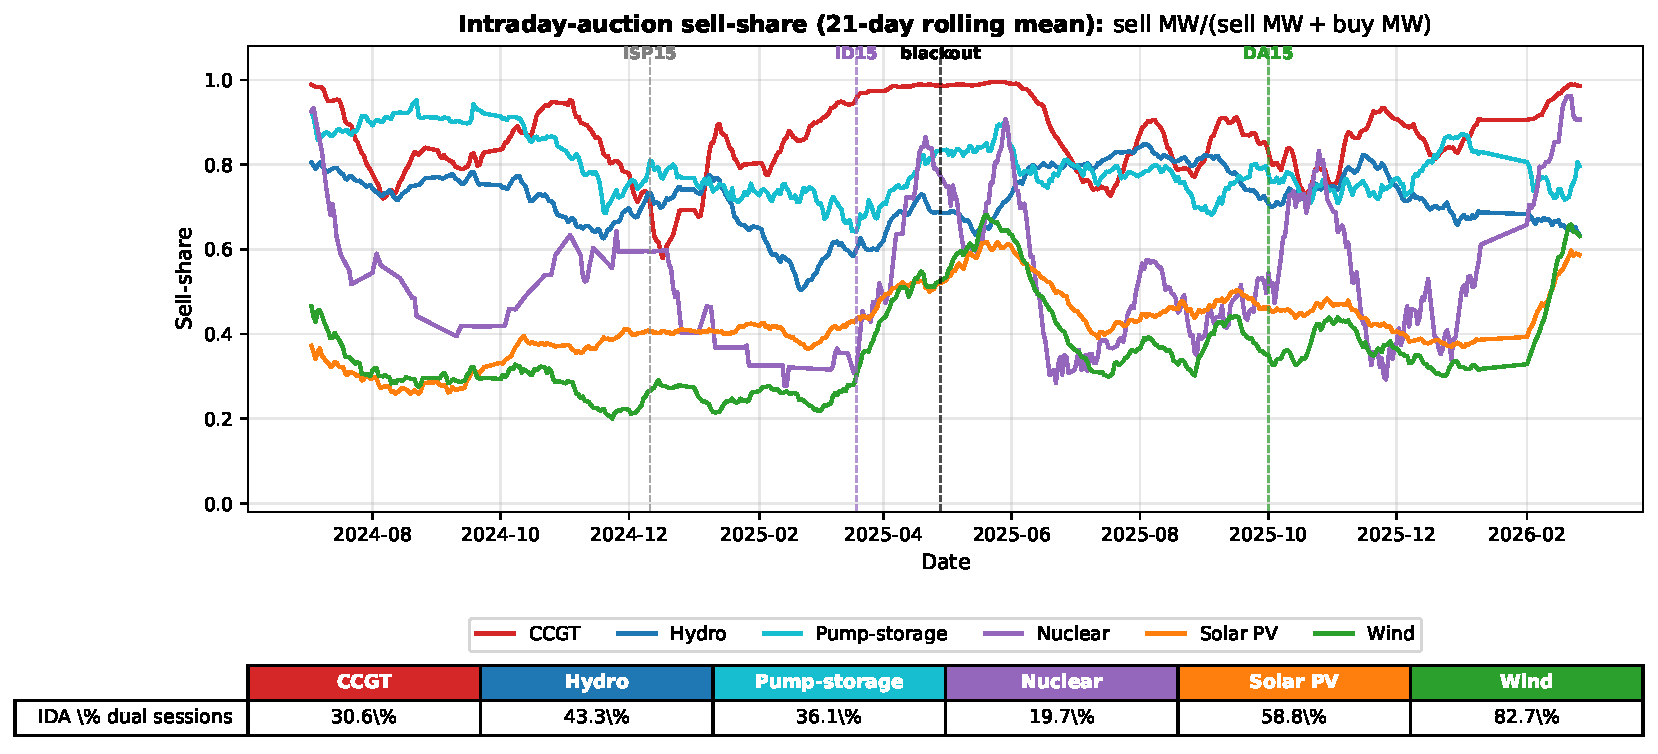
\includegraphics[width=\linewidth]{fig_sell_share_over_time.pdf}\\[-0.05cm]
\footnotesize
IDA sell-share by technology, $21$-day rolling. Vertical: reform cutovers. Generators submit BOTH buy and sell orders within the same IDA session $\Rightarrow$ they actively arbitrage their own DA position. The level shifts at March~2025.
\end{column}
\begin{column}{0.45\textwidth}
\footnotesize
\textbf{BSTS sell-share change at ID15 (pp)} --- long-pre Spec~A with renewables and gas controls.
\medskip
\centering
\setlength{\tabcolsep}{4pt}
\begin{tabular}{l c}
\toprule
\textbf{Technology} & $\hat\Delta$ (pp) \\
\midrule
\rowcolor{green!22} Nuclear     & $\mathbf{33.5}^{***}$ \\
\rowcolor{green!22} Wind        & $\mathbf{23.5}^{***}$ \\
Hydro                & $4.8^{***}$ \\
Solar PV             & $3.6^{**}$ \\
\rowcolor{red!12} Pumped hydro & $3.9$ \\
\rowcolor{red!12} CCGT         & $-3.1$ \\
\bottomrule
\end{tabular}

\medskip
\raggedright
\textcolor{green!40!black}{\textbf{Nuclear and wind} swing into selling.} Pre-reform they used IDA as a one-way buy market; post-March they actively price output at 15-min resolution. CCGT (strategic-bidder benchmark) does NOT shift its DA/IDA mix.
\end{column}
\end{columns}
\end{frame}


% ---------------------------------------------------------------------------
\begin{frame}{Cleared quantities --- OLS per technology, both reforms}
\footnotesize
\textbf{OLS spec.} Daily cleared GWh per (tech, market). Same RHS as the price spec; Newey-West HAC. Two cells per tech: \emph{ID15 IDA} (granular venue at the IDA reform) and \emph{DA15 DA} (granular venue at the DA reform).

\medskip
\centering
\setlength{\tabcolsep}{6pt}
\begin{tabular}{l r c r c}
\toprule
                  & \multicolumn{2}{c}{\textbf{ID15 IDA cleared (PIBCI)}} & \multicolumn{2}{c}{\textbf{DA15 DA cleared (PDBC)}} \\
\cmidrule(lr){2-3}\cmidrule(lr){4-5}
\textbf{Tech}     & \textbf{$\hat\theta$ (GWh/day)} & \textbf{p} & \textbf{$\hat\theta$ (GWh/day)} & \textbf{p} \\
\midrule
CCGT              & \cellcolor{red!12}$\mathbf{-5.5}^{***}$  & 0.002 & $14$              & 0.24 \\
Hydro             & \cellcolor{red!12}$\mathbf{-3.8}^{**}$   & 0.02  & \cellcolor{red!12}$\mathbf{-8.5}^{***}$ & 0.000 \\
Pumped hydro      & \cellcolor{red!12}$-0.6^{*}$             & 0.05  & \cellcolor{green!22}$\mathbf{3.4}^{**}$ & 0.003 \\
Nuclear           & $3.7$                                   & 0.62  & \cellcolor{green!22}$\mathbf{27}^{*}$  & 0.07 \\
Solar             & \cellcolor{green!22}$\mathbf{6.3}^{***}$ & 0.000 & \cellcolor{green!22}$\mathbf{6.5}^{***}$ & 0.000 \\
Wind              & \cellcolor{green!22}$\mathbf{3.9}^{***}$ & 0.008 & \cellcolor{green!22}$\mathbf{11}^{**}$  & 0.015 \\
\bottomrule
\end{tabular}

\medskip
\raggedright
\begin{itemize}\setlength{\itemsep}{1pt}
  \item \textcolor{green!40!black}{\textbf{Renewables flow toward the granular venue at each reform.}} ID15: solar $+6.3$ and wind $+3.9$ GWh/day INTO IDA. DA15: solar $+6.5$, wind $+11$ GWh/day INTO DA. Direction matches the model's aggregator-on-granular-leg prediction.
  \item \textcolor{red!70!black}{\textbf{Dispatchable techs lose share on the IDA at ID15:}} CCGT $-5.5$ and hydro $-3.8$ GWh/day. At DA15 the DA side scales up across the board (pump-storage, nuclear, wind).
  \item BSTS cross-check: same qualitative pattern (CCGT IDA $-8$, solar IDA $+6.7$, wind IDA $+5.3$ at ID15; solar DA $+11$ at ID15; CCGT DA $+36$, wind DA $+18$ at DA15).
\end{itemize}
\end{frame}


% ---------------------------------------------------------------------------
\begin{frame}{Penalty --- imbalance per MWh drops; aggregate volume does not}
\footnotesize
\textbf{Setup.} Parties that deviate from contract pay a regulated penalty per MWh of deviation.

\smallskip
\textbf{BSTS spec.} $\hat\Delta = \tfrac{1}{T_{\text{post}}}\sum_{t\in\text{post}}\!\big(Y_t - \hat Y_t^{\text{cf}}\big)$ on daily outcomes, with (wind, solar, gas) regressors and 2022$-$present seasonality.

\medskip
\centering
\setlength{\tabcolsep}{10pt}
\begin{tabular}{l c c}
\toprule
\textbf{Outcome} & \textbf{March reform} & \textbf{October reform} \\
\midrule
Penalty per MWh of deviation         & \cellcolor{green!22}$\mathbf{-33}\%^{***}$ & \cellcolor{red!12}flat \\
Aggregate imbalance volume (MWh/day) & \cellcolor{red!12}$-0.1\%$        & \cellcolor{red!12}$-4\%$ \\
\bottomrule
\end{tabular}

\medskip
\raggedright
\begin{itemize}\setlength{\itemsep}{2pt}
  \item \textcolor{green!40!black}{\textbf{Main finding (green):} penalty per MWh falls by a third at March.} The granular spot lets the operator price-discriminate the residual imbalance at a lower marginal cost.
  \item \textcolor{red!70!black}{\textbf{Negative findings (red):}}
    \begin{itemize}\setlength{\itemsep}{1pt}
      \item Aggregate imbalance volume does NOT drop $\Rightarrow$ granularity reorganises the \emph{within-hour} composition of imbalance, not the size of aggregate forecast errors.
      \item Penalty per MWh is flat at October $\Rightarrow$ the gain was captured at the IDA reform; the DA reform adds no further compression.
    \end{itemize}
\end{itemize}
\end{frame}


% ---------------------------------------------------------------------------
\subsection{Bid shape and residual demand slope}

\begin{frame}{Bid shape --- CCGT ladders widen in critical hours (Spec C)}
\footnotesize
\textbf{DiD spec.} For each (reform, venue) cell, per-curve fit:
\[
Y_{u,d,p} \;=\; \theta\,\mathds{1}\{d \in \text{post}\}\cdot\mathds{1}\{p \in \text{crit}\} \;+\; \alpha_u \;+\; \phi_p \;+\; \delta_d \;+\; \varepsilon_{u,d,p},
\]
with critical hours as treated and flat hours as the within-day falsifier. Table reports $\theta$.

\medskip
\centering
\setlength{\tabcolsep}{6pt}
\begin{tabular}{l c c c c}
\toprule
                       & \multicolumn{2}{c}{\textbf{March (IDA reform)}} & \multicolumn{2}{c}{\textbf{October (DA reform)}} \\
\cmidrule(lr){2-3} \cmidrule(lr){4-5}
\textbf{DiD $\theta$} & DA & IDA & DA & IDA \\
\midrule
$\sigma_p$ (EUR/MWh)              & \cellcolor{orange!18}$\mathbf{4.17}^{***}$ & \cellcolor{red!12}$0.10$            & \cellcolor{green!22}$\mathbf{0.68}^{***}$  & $-0.68^{*}$ \\
$\hat\alpha$ (EUR/MWh)            & \cellcolor{orange!18}$\mathbf{-40.2}^{***}$ & $11.8^{*}$        & \cellcolor{green!22}$\mathbf{28.3}^{***}$  & $6.0^{**}$ \\
$\hat\beta$ (EUR/MWh per MW)      & \cellcolor{orange!18}$\mathbf{0.27}^{***}$ & $-0.88^{*}$        & \cellcolor{green!22}$\mathbf{-0.15}^{***}$  & \cellcolor{red!12}$0.20$ \\
$\hat\gamma$ ($\times 10^{3}$)    & \cellcolor{orange!18}$\mathbf{-3.99}^{***}$ & \cellcolor{red!12}$10.0$            & \cellcolor{green!22}$\mathbf{1.03}^{***}$  & $7.6$ \\
$\text{HHI}_p$                    & \cellcolor{orange!18}$\mathbf{-0.076}^{***}$ & $\mathbf{-0.041}^{***}$ & \cellcolor{green!22}$\mathbf{-0.059}^{***}$ & $\mathbf{0.051}^{***}$ \\
\bottomrule
\end{tabular}

\medskip
\raggedright
\footnotesize
\begin{itemize}\setlength{\itemsep}{2pt}
  \item \textcolor{green!40!black}{\textbf{Main finding (green):} DA at October.} $\sigma_p$ rises, $\hat\alpha$ lifts, $\hat\beta$ flattens, $\hat\gamma$ bends convex, $\text{HHI}_p$ falls. Bid stack \emph{deconcentrates}: more MW packed cheap at low quantities (Cournot scale-up) plus a steeper tail above the clearing price.
  \item \textcolor{orange!50!black}{\textbf{Anticipation (orange):} DA at March} --- opposite curvature sign $\Rightarrow$ different mechanism (anticipating the IDA reform).
  \item \textcolor{red!70!black}{\textbf{Null findings (red):} $\sigma_p$ and $\hat\gamma$ at the March IDA reform; $\hat\beta$ at the October IDA.} The reformed venue does not restructure on its own reform date.
\end{itemize}
\end{frame}


% ---------------------------------------------------------------------------
\begin{frame}{Residual demand slope --- per-firm Cournot competitiveness rises on the reformed venue}
\footnotesize
\textbf{Object.} For each of the four dominant generators, the slope $b_{m,t}$ of the residual demand it faces (Cournot primitive). Steeper $\Rightarrow$ less unilateral market power.

\smallskip
\textbf{DiD spec (per firm, per reform $\times$ venue).}
\[
\log\, b_{f,t} \;=\; \theta_f\,\mathds{1}\{t \in \text{post}\} \;+\; \text{month FE} \;+\; \text{(wind, solar daily)} \;+\; \varepsilon_{f,t}.
\]
Table reports $\theta_f$ (\% change in slope).

\medskip
\centering
\setlength{\tabcolsep}{8pt}
\begin{tabular}{l c c c c}
\toprule
\textbf{Change in slope per firm} & Firm 1 & Firm 2 & Firm 3 & Firm 4 \\
\midrule
March reform, slope on IDA           & \cellcolor{green!22}$10\%$ & \cellcolor{green!22}$13\%$ & \cellcolor{green!22}$\mathbf{17}\%^{*}$ & \cellcolor{green!22}$13\%$ \\
October reform, slope on IDA         & \cellcolor{green!22}$11\%$ & \cellcolor{green!22}$13\%$ & \cellcolor{green!22}$12\%$              & \cellcolor{green!22}$\mathbf{15}\%^{***}$ \\
October reform, slope on DA          & \cellcolor{red!12}$-2\%$  & \cellcolor{red!12}$-1\%$  & \cellcolor{red!12}$-2\%$               & \cellcolor{red!12}$-3\%$ \\
\bottomrule
\end{tabular}

\medskip
\raggedright
\begin{itemize}\setlength{\itemsep}{2pt}
  \item \textcolor{green!40!black}{\textbf{Main finding (green):} slope thickens on the IDA side at both reforms.} Direction consistent for every firm; wind/solar daily-production controls barely move the coefficient $\Rightarrow$ not a supply-shift artefact.
  \item \textcolor{red!70!black}{\textbf{Negative finding (red):} DA at October.} The newly-reformed DA does NOT thicken its own slope. Effect is venue-specific to the IDA side.
\end{itemize}
\end{frame}


% ---------------------------------------------------------------------------
\begin{frame}{The April 2025 blackout triggered a separate regulatory regime}
\begin{center}
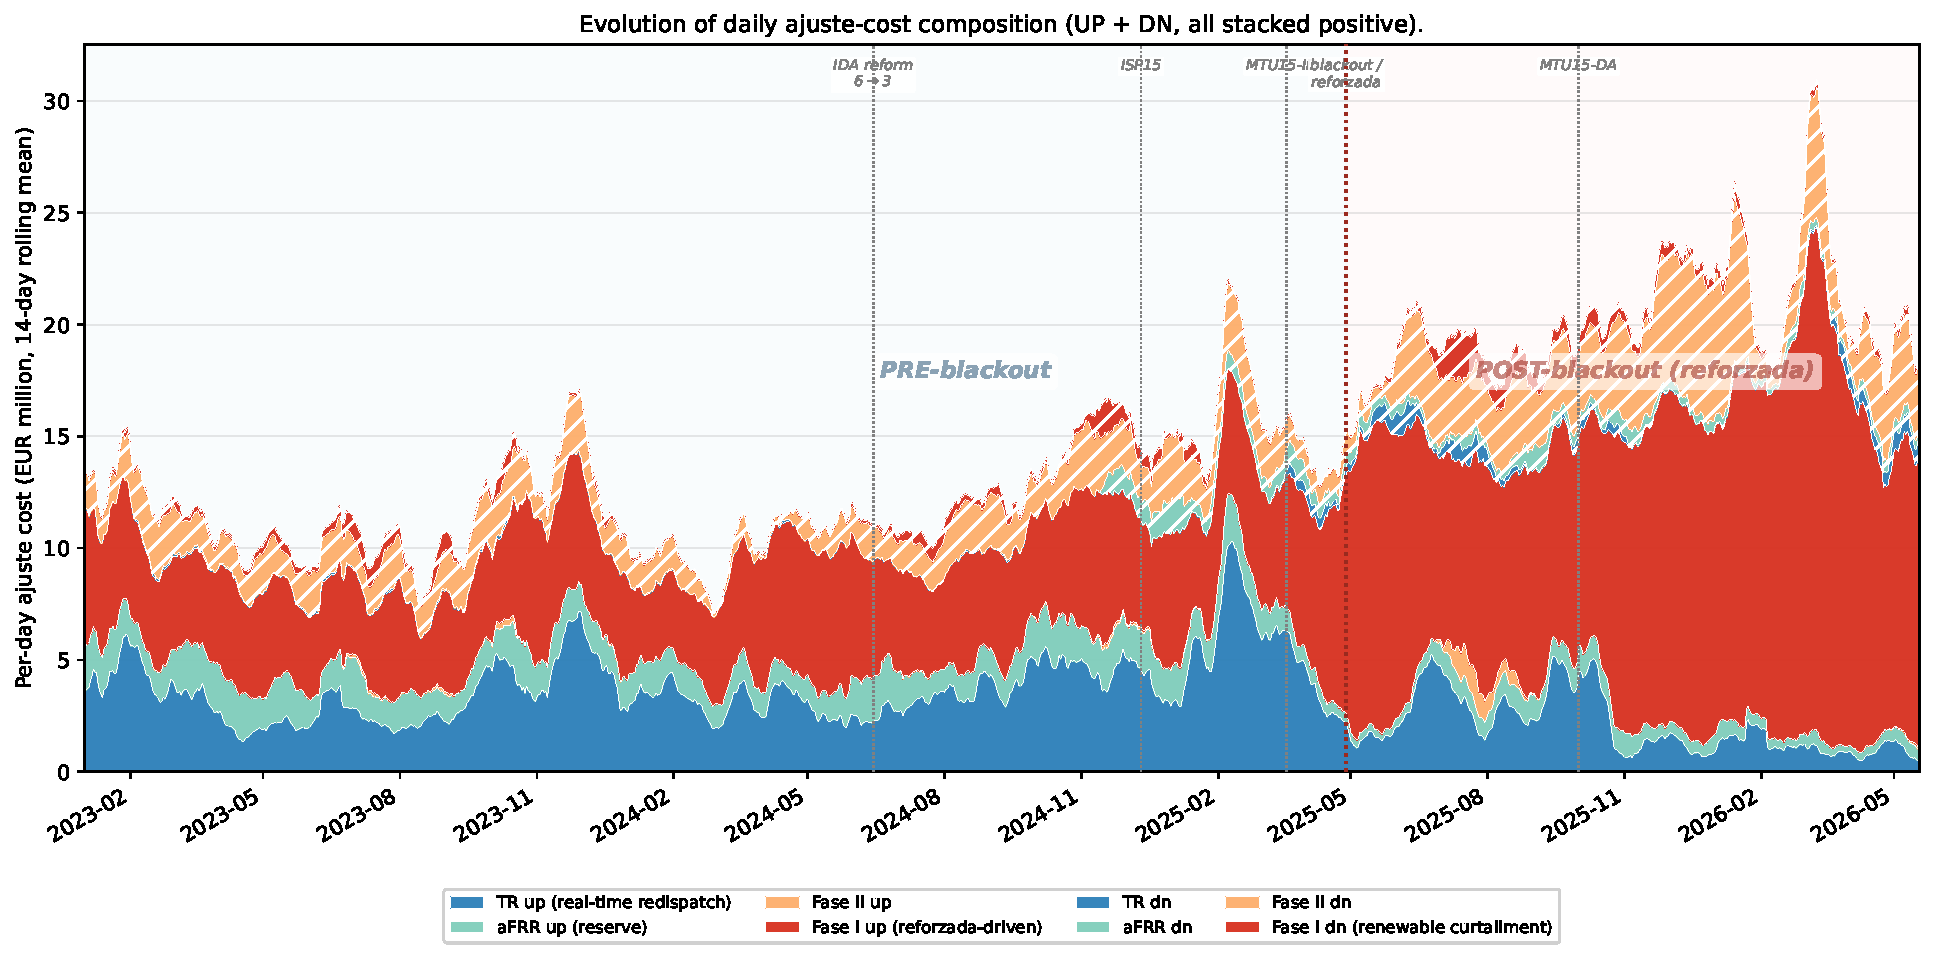
\includegraphics[width=0.72\linewidth]{efficiency_gains_timeseries.pdf}
\end{center}
\vspace{-0.1cm}
\footnotesize
\begin{itemize}\setlength{\itemsep}{2pt}
  \item Post-blackout, the system operator keeps combined-cycle gas plants synchronised for voltage support, paid through a separate redispatch channel ($+5$M EUR/day). Daily technical-restrictions cost: $2.4 \to 10.7$ M EUR.
  \item \textcolor{red!70!black}{\textbf{Negative finding:}} the real-time TR/aFRR cost decrease is largely \emph{timing displacement} from real-time to Fase\,I within the post-blackout regime, \emph{not} a granularity efficiency gain.
  \item \textbf{Nuclear and gas at March 2025.} In the 40 days between the IDA reform and the blackout, nuclear's auction-plus-bilateral output drops sharply against a same-calendar 2024 placebo --- the granular leg sharpens bidding, DA prices run very low on solar-heavy days, and inflexible nuclear baseload loses room. Post-blackout, CCGT roughly doubles its restriction dispatch to provide voltage support. Triangulated by Davi-Arderius \& Graf (2026).
  \item \textbf{Take away.} Granularity and the post-blackout regime overlap on the calendar but operate on different mechanisms. The cost rise belongs to the post-blackout regime.
\end{itemize}
\end{frame}

\section{Conclusion}

\begin{frame}{Conclusion}

\end{frame}

% ---------------------------------------------------------------------------
\begin{frame}[plain]
\begin{center}
\vfill
{\Huge\bfseries\color{blue!50!black} Thank you.}\\[1.2cm]
{\Large\color{blue!50!black} Questions?}
\vfill
\end{center}
\end{frame}

\begin{frame}[allowframebreaks]{References}
\scriptsize
\bibliography{../../paper/references}
\end{frame}

% ===========================================================================
% APPENDIX SLIDES (Q\&A)
% ===========================================================================


\section{Appendix}

\begin{frame}{ID15 price effect at longer post-windows}
\footnotesize
\centering
\setlength{\tabcolsep}{8pt}
\begin{tabular}{l c c c c}
\toprule
                                     & \textbf{40 d}$^{\dagger}$ & \textbf{90 d} & \textbf{180 d} & \textbf{196 d}$^{\ddagger}$ \\
\midrule
\multicolumn{5}{l}{\emph{OLS daily, ID15 IDA price (EUR/MWh, Newey-West HAC lag=7)}} \\
\hspace{0.5em}base (month $+$ DOW)               & $-32^{***}$ & $-37^{***}$ & $-25^{***}$ & $-25^{***}$ \\
\hspace{0.5em}$+$ year-by-renew (per year)       & $-46^{***}$ & $-53^{***}$ & $-54^{***}$ & $-53^{***}$ \\
\hspace{0.5em}$+$ year-by-renew (2024+25 pooled) & \cellcolor{green!22}$\mathbf{-39}^{***}$ & \cellcolor{green!22}$\mathbf{-42}^{***}$ & \cellcolor{green!22}$\mathbf{-30}^{***}$ & \cellcolor{green!22}$\mathbf{-30}^{***}$ \\
\addlinespace
\multicolumn{5}{l}{\emph{OLS hourly, ID15 IDA price (EUR/MWh, Newey-West HAC lag=24$\times$7)}} \\
\hspace{0.5em}base (hour $+$ month $+$ DOW)      & $-34^{***}$ & $-38^{***}$ & $-25^{***}$ & $-25^{***}$ \\
\hspace{0.5em}$+$ year-by-renew (per year)       & $-40^{***}$ & $-43^{***}$ & $-31^{***}$ & $-31^{***}$ \\
\hspace{0.5em}$+$ year-by-renew (2024+25 pooled) & \cellcolor{green!22}$\mathbf{-30}^{***}$ & \cellcolor{green!22}$\mathbf{-35}^{***}$ & \cellcolor{green!22}$\mathbf{-24}^{***}$ & \cellcolor{green!22}$\mathbf{-24}^{***}$ \\
\addlinespace
\multicolumn{5}{l}{\emph{BSTS daily, ID15 IDA price (per-year long-pre spec)}} \\
\hspace{0.5em}Real effect                        & \cellcolor{green!22}$-34^{*}$ & \cellcolor{green!22}$-35$ & $-12$ & $-10$ \\
\bottomrule
\end{tabular}

\smallskip
{\scriptsize\itshape $^{\dagger}$Pre-blackout headline window. $^{\ddagger}$Up to DA15 cutover (max ID15 post not contaminated by DA15). All specs significant at $p<0.01$ on the OLS rows. ID15 DA cross-market estimates are within $\pm 1$ EUR/MWh of the ID15 IDA own-venue values at every cell.}
\end{frame}

% ---------------------------------------------------------------------------

\begin{frame}{Price effect by hour class}
\footnotesize
\centering
OLS hourly $+$ year-by-renewable (2024$+$25 pooled) spec, pre-window 2022-01-01 onward. Newey-West HAC lag\,$=24\times 7$. Same headline post-windows (ID15 40 d, DA15 92 d).

\medskip
\setlength{\tabcolsep}{10pt}
\begin{tabular}{l c c c c}
\toprule
\textbf{Hour class}              & \textbf{ID15 IDA} & \textbf{ID15 DA cross} & \textbf{DA15 DA} & \textbf{DA15 IDA cross} \\
\midrule
Morning ramp (5--8)              & \cellcolor{green!22}$-33^{**}$ & \cellcolor{green!22}$-32^{*}$ & \cellcolor{red!18}$3$  & \cellcolor{red!18}$1$ \\
Evening ramp (16--22)            & \cellcolor{green!22}$-25^{*}$  & \cellcolor{green!22}$-24^{*}$  & \cellcolor{red!18}$1$  & \cellcolor{red!18}$-1$ \\
Midday (11--14)                  & \cellcolor{green!22}$\mathbf{-39}^{***}$ & \cellcolor{green!22}$\mathbf{-37}^{***}$ & \cellcolor{red!18}$-3$ & \cellcolor{red!18}$-5$ \\
Flat (1--3)                      & \cellcolor{green!22}$-34^{**}$ & \cellcolor{green!22}$-30^{*}$  & \cellcolor{red!18}$2$  & \cellcolor{red!18}$3$ \\
\bottomrule
\end{tabular}

\bigskip
\textbf{Reading.} \textcolor{green!40!black}{\textbf{ID15 price drop is broadly uniform across hour classes}} ($-25$ to $-39$ EUR/MWh) and slightly larger at midday (when solar saturation pushes prices low, the granular leg helps integrate flexibility most). \textcolor{red!70!black}{\textbf{DA15 null everywhere}} --- no hour-class heterogeneity rescues the headline DA15 null.
\end{frame}

% ---------------------------------------------------------------------------

\begin{frame}{Placebo prices table}
\footnotesize
Same row structure as the headline prices table; cutovers shifted to \emph{2024-03-19} (ID15 placebo, 40 d post) and \emph{2024-10-01} (DA15 placebo, 92 d post). Same pre-window 2022-01-01 onward.

\medskip
\centering
\setlength{\tabcolsep}{4pt}
\begin{tabular}{l c c c c}
\toprule
                                                   & \multicolumn{2}{c}{\textbf{ID15 placebo (cut.\ 2024-03-19)}} & \multicolumn{2}{c}{\textbf{DA15 placebo (cut.\ 2024-10-01)}} \\
\cmidrule(lr){2-3}\cmidrule(lr){4-5}
                                                   & IDA & DA cross & DA & IDA cross \\
\midrule
OLS daily --- base (month $+$ DOW)                   & \cellcolor{red!22}$-49^{***}$ & \cellcolor{red!22}$-50^{***}$ & \cellcolor{green!22}$10$ & \cellcolor{green!22}$12$ \\
OLS daily --- $+$ year-by-renewable (per year)       & \cellcolor{green!22}$2$ & \cellcolor{green!22}$1$ & \cellcolor{red!22}$50^{***}$ & \cellcolor{red!22}$50^{***}$ \\
OLS daily --- $+$ year-by-renewable (2024+25 pooled) & \cellcolor{green!22}$2$ & \cellcolor{green!22}$1$ & \cellcolor{red!22}$50^{***}$ & \cellcolor{red!22}$50^{***}$ \\
\addlinespace
OLS hourly --- base (hour $+$ month $+$ DOW)         & \cellcolor{red!22}$-49^{***}$ & \cellcolor{red!22}$-49^{***}$ & \cellcolor{green!22}$9$ & \cellcolor{green!22}$11$ \\
OLS hourly --- $+$ year-by-renewable (per year)      & \cellcolor{green!22}$-11$ & \cellcolor{green!22}$-12$ & \cellcolor{red!22}$47^{***}$ & \cellcolor{red!22}$48^{***}$ \\
OLS hourly --- $+$ year-by-renewable (2024+25 pooled)& \cellcolor{green!22}$-11$ & \cellcolor{green!22}$-12$ & \cellcolor{red!22}$47^{***}$ & \cellcolor{red!22}$48^{***}$ \\
\addlinespace
BSTS daily                                           & \cellcolor{green!22}$-22$ & \cellcolor{green!22}$-15$ & \cellcolor{green!22}$4$ & \cellcolor{green!22}$27$ \\
\bottomrule
\end{tabular}

\end{frame}


% ---------------------------------------------------------------------------


\begin{frame}{Per-IDA-session price effect breakdown}
\footnotesize
\centering
Pre-window 2024-06-14 onward (European-IDA 3-session regime); year-by-renewable 2024+25 pooled spec; Newey-West HAC SE (lag\,$=7$ daily, $24\times7$ hourly).

\medskip
\setlength{\tabcolsep}{10pt}
\begin{tabular}{l c c c}
\toprule
\textbf{Session}                                  & S1 (early) & S2 (mid) & S3 (late) \\
\midrule
ID15 own-venue effect (EUR/MWh) --- OLS daily     & \cellcolor{green!22}$\mathbf{-37}^{***}$ & \cellcolor{green!22}$\mathbf{-35}^{***}$ & \cellcolor{green!22}$\mathbf{-29}^{***}$ \\
ID15 own-venue effect (EUR/MWh) --- OLS hourly    & \cellcolor{green!22}$\mathbf{-39}^{***}$ & \cellcolor{green!22}$\mathbf{-37}^{***}$ & \cellcolor{green!22}$\mathbf{-34}^{***}$ \\
\addlinespace
DA15 cross-market effect --- OLS daily            & \cellcolor{red!18}$14$  & \cellcolor{red!18}$17^{*}$ & \cellcolor{red!18}$11$ \\
DA15 cross-market effect --- OLS hourly           & \cellcolor{red!18}$18$  & \cellcolor{red!18}$23^{*}$ & \cellcolor{red!18}$13$ \\
\bottomrule
\end{tabular}

\bigskip
\textbf{Reading.} \textcolor{green!40!black}{ID15 price drop is uniform across sessions} ($-34$ to $-39$ EUR/MWh under hourly) --- the granular-leg discount is not concentrated in any one session. \textcolor{red!70!black}{DA15 cross-effect on IDA sessions is positive but mostly null}, consistent with the DA-own-venue null on the headline slide.
\end{frame}


% ---------------------------------------------------------------------------


\begin{frame}{Price wedges placebos}
  
\end{frame}


% ---------------------------------------------------------------------------
\begin{frame}{Program cascade for other technologies}
\centering
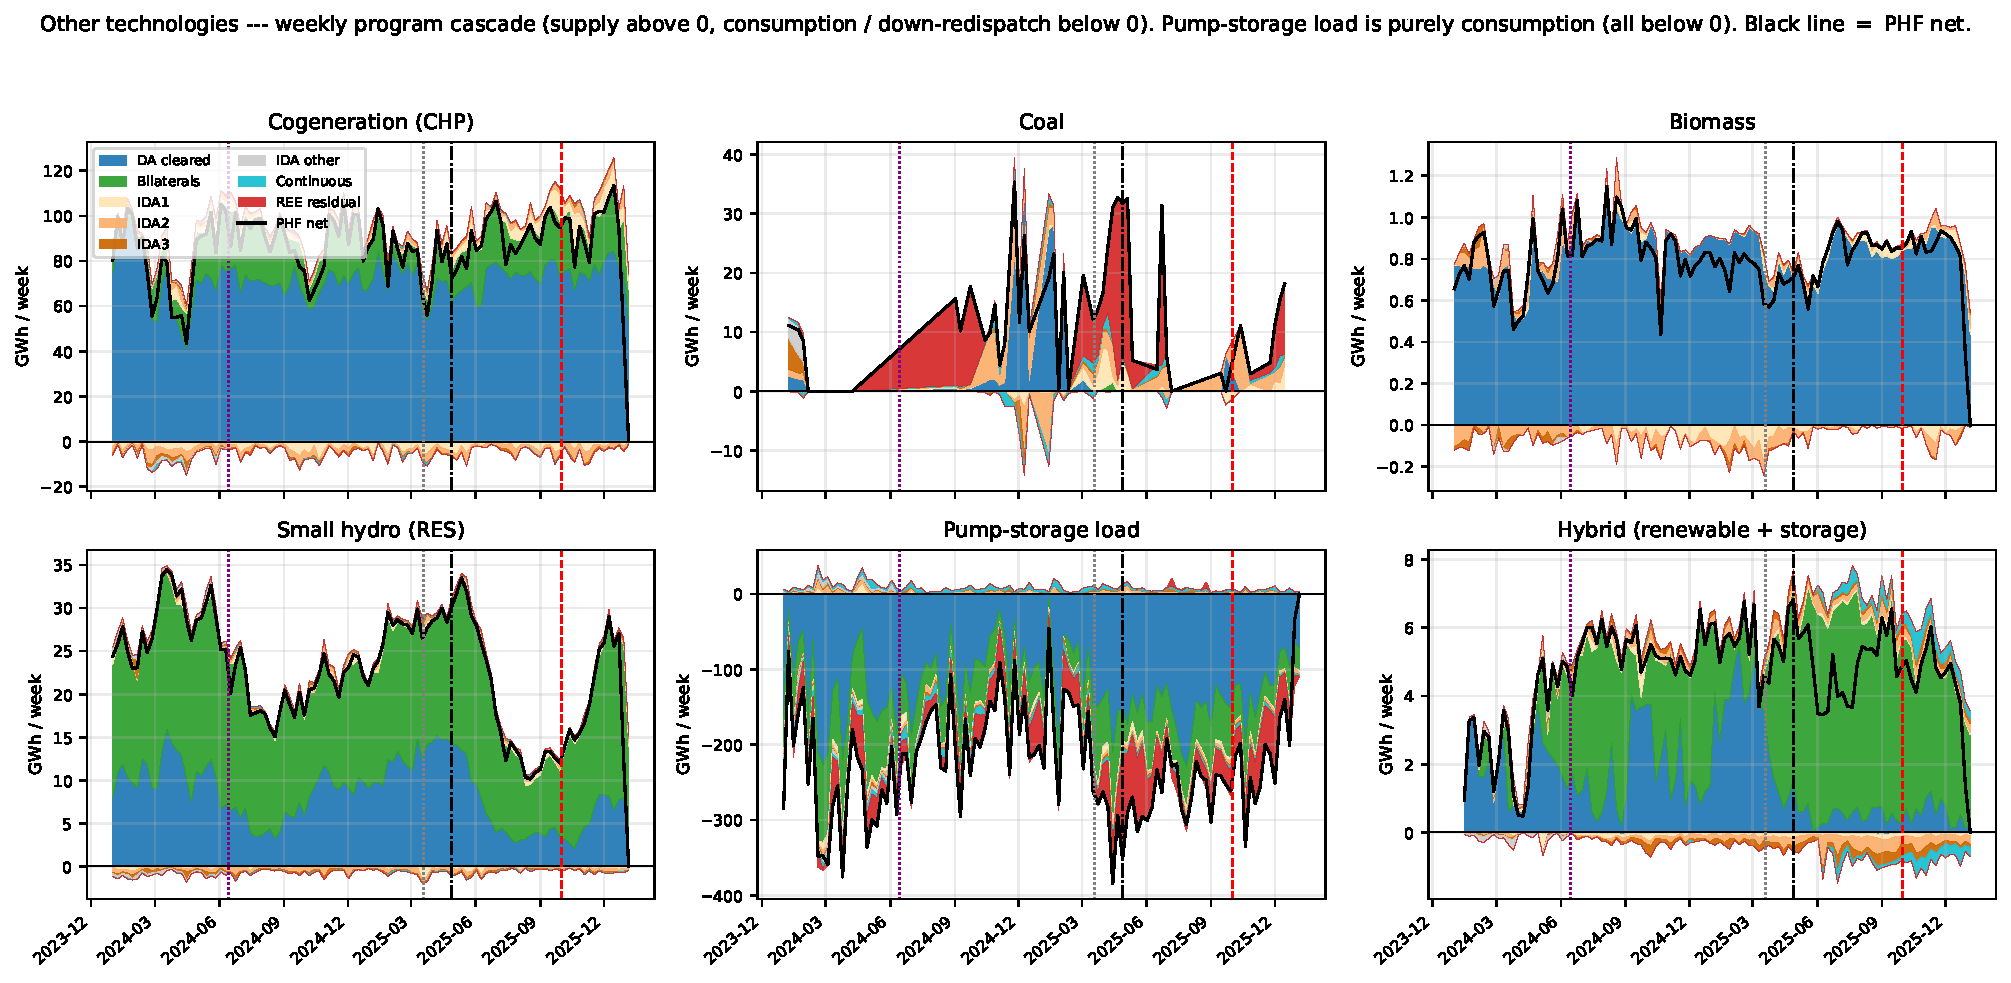
\includegraphics[width=0.95\linewidth]{fig_programs_by_tech_other_weekly.pdf}
\end{frame}

% ---------------------------------------------------------------------------

\begin{frame}
  
\end{frame}


% ---------------------------------------------------------------------------


\begin{frame}{Appendix --- In-band offered energy migrates to the granular market}
\centering
\footnotesize
\setlength{\tabcolsep}{4pt}
\begin{tabular}{l l r r r r}
\toprule
              &               & \multicolumn{2}{c}{\textbf{ID15 (Net, MWh/class-hr)}} & \multicolumn{2}{c}{\textbf{DA15 (Net, MWh/class-hr)}} \\
\cmidrule(lr){3-4} \cmidrule(lr){5-6}
\textbf{Tech} & \textbf{Hour class} & DA & IDA & DA & IDA \\
\midrule
CCGT          & morning ramp  & $77$               & $\mathbf{2090}^{***}$ & $\mathbf{3462}^{**}$  & $\mathbf{-1627}^{***}$ \\
              & midday        & $-1497^{***}$      & $\mathbf{1426}^{***}$ & $988^{**}$             & $773^{*}$ \\
              & evening ramp  & $191$              & $\mathbf{1859}^{***}$ & $\mathbf{2458}^{***}$ & $-152$ \\
              & flat          & $-863^{**}$        & $\mathbf{1405}^{***}$ & $\mathbf{2966}^{**}$  & $\mathbf{-1157}^{***}$ \\
Pump-storage  & midday        & $151$              & $\mathbf{979}^{**}$   & $\mathbf{433}^{**}$   & $\mathbf{868}^{**}$ \\
              & evening ramp  & $-1$               & $\mathbf{775}^{*}$    & $251$                  & $-408$ \\
\bottomrule
\end{tabular}

\bigskip
CHECK HERE WHAT WE ARE DOING!!!
\footnotesize
\begin{itemize}\setlength{\itemsep}{2pt}
  \item Under ID15, CCGT and pump-storage push energy \emph{into} IDA (the granular leg); under DA15, they push it back into DA.
  \item Hydro is the exception (reservoir-driven, 2024 placebo poor); not leaned on.
  \item Bid-side primitive of the cleared scale-up in critical hours under DA15.
\end{itemize}
\end{frame}

% ---------------------------------------------------------------------------
\begin{frame}{Appendix --- Bid-shape parallel trends (visual check)}
\begin{center}
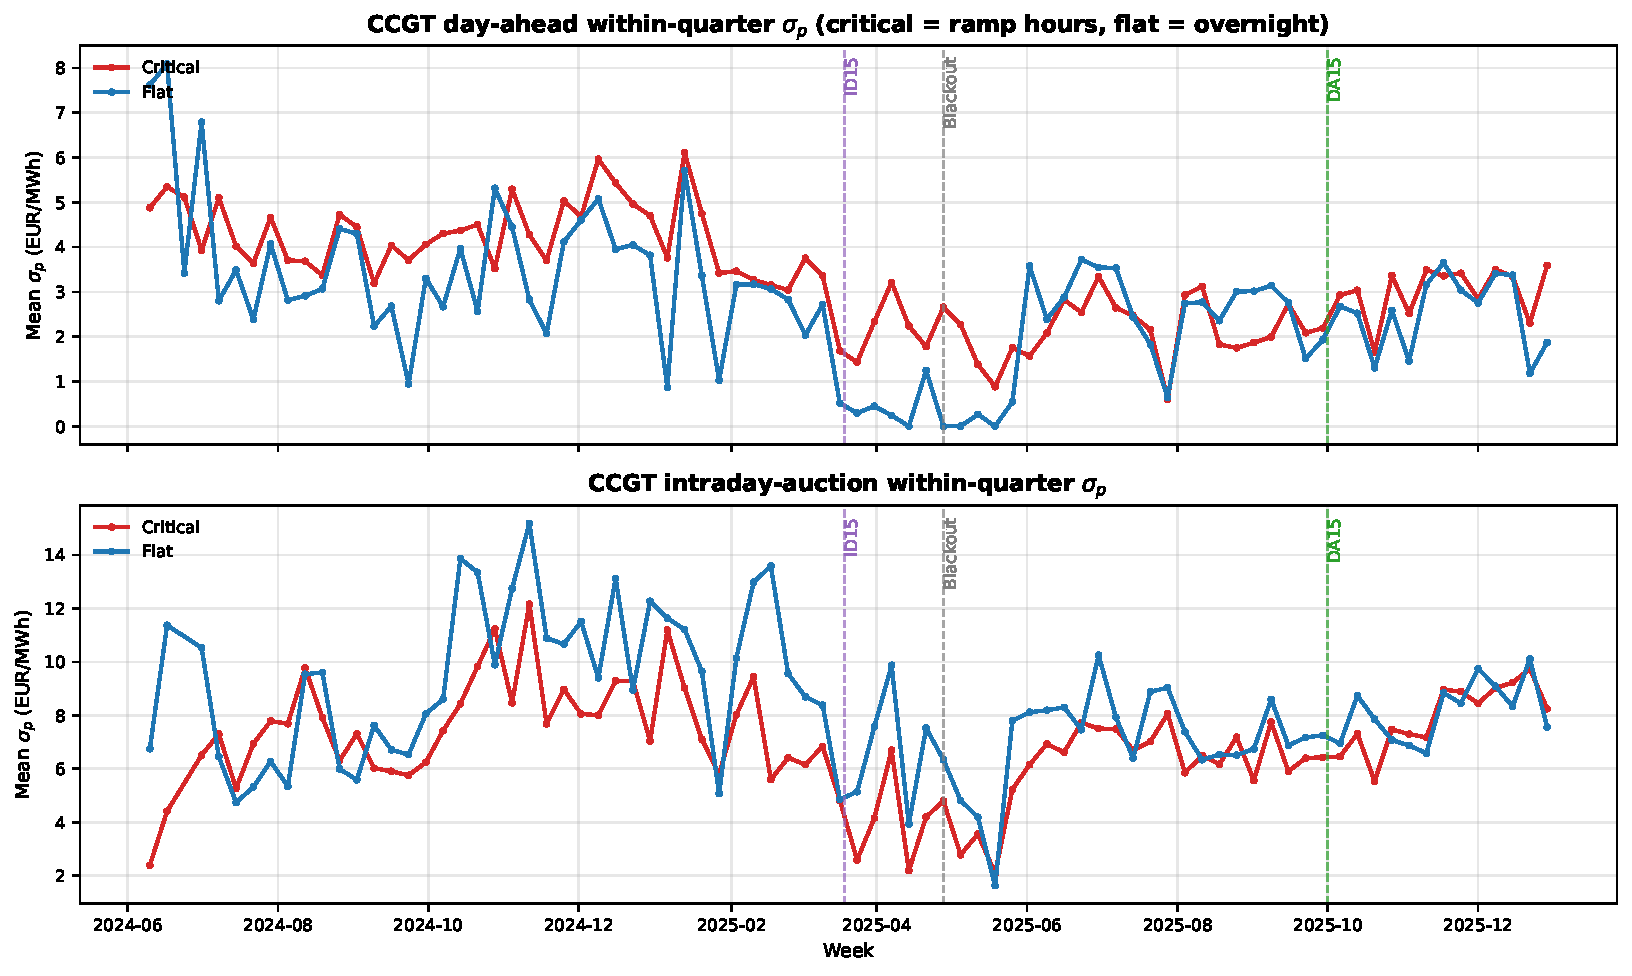
\includegraphics[width=0.84\linewidth]{fig_parallel_trends_sigma_p.pdf}
\end{center}

\footnotesize
\begin{itemize}\setlength{\itemsep}{2pt}
  \item Critical $-$ flat differential of $\sigma_p$, weekly resolution, by tech-market cell.
  \item Pre-reform: trends visually flat (no anticipation drift).
  \item Jump at the reform cutover; persistence post-reform.
\end{itemize}
\end{frame}




% ---------------------------------------------------------------------------


% ---------------------------------------------------------------------------
\begin{frame}

\end{frame}

% ---------------------------------------------------------------------------


% ---------------------------------------------------------------------------


\end{document}
